\section{Méthode proposée}
La méthode proposée par l'article \cite{farbman2011tonal} se décompose en un certain nombre d'étapes qui seront décrites dans ce chapitre.

\subsection{Sélection d'images de références}
Afin de réaliser la stabilisation tonale de la séquence d'image, l'utilisateur doit choisir une (ou des) image de référence. Ces images sont les images que l'utilisateur choisit comme référence de tonalité. 
Les auteurs proposent de choisir des images de références par paires, ces paires délimitant des parties de la séquence dans lesquelles une importante variation de la tonalité a lieu.
 
\subsection{Lissage avec préservation des bordures}
Dans un second temps, un lissage des images avec un filtre préservant les bordures est appliqué. Cela a pour impact d'atténuer les variations qui ne proviennent pas des paramètres de tonalité de la caméra. 

\begin{figure}[h]
\centering
\begin{tabular}{cc}
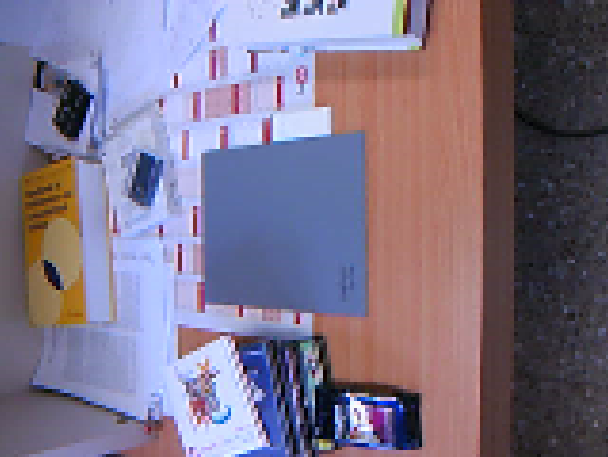
\includegraphics[width = 0.4\textwidth]{Chapters/Images/bilteral_filter1.png}&
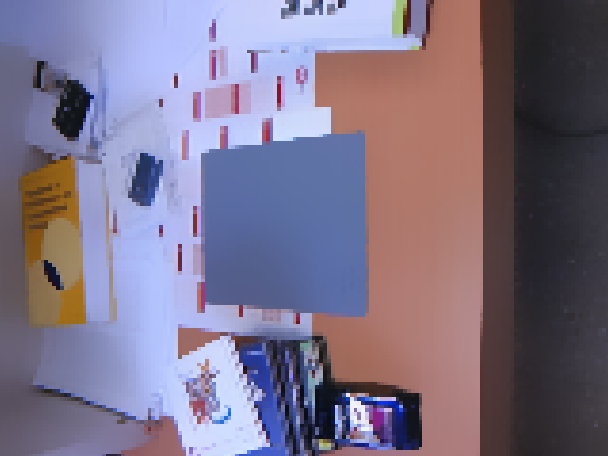
\includegraphics[width = 0.4\textwidth]{Chapters/Images/bilteral_filter2.png}
\end{tabular}
\caption{Left : Image d'origine sous échantillonnée, Right : Filtre bilatéral avec les paramètres recommandés}
\end{figure}

\subsection{Mise en correspondances de pixels}
Comme, dans une vidéo, les images sont cohérentes spatialement et temporellement, une grande partie des pixels de l'image peuvent être mis en correspondances. Afin de réaliser cela, les auteurs proposent d'utiliser la luminance de deux images consécutives afin de sélectionner ces pixels.

A partir des composantes R,G,B d'une image, la luminance peut s'écrire sous la forme $L = 0,299 R + 0,587 G + 0,114 B$. Les auteurs proposent de conserver dans l'ensemble des correspondances (\textit{robust set}) les pixels dont la luminance a peu changé entre deux images successives. Cette condition est exprimée par l'équation \ref{eqn_robust}

\begin{equation}
R_{i/i+1} = \left\{x \: s.t. |(L_{i}(x)-\mu(L_{i})) - (L_{i+1}(x)-\mu(L_{i+1}))| < 0.05 \right\}
\label{eqn_robust}
\end{equation}

On peut observer sur l'image \ref{fig_robust} le \textit{robust set} créé à partir de deux images successives.

\begin{figure}[H]
\centering
\begin{tabular}{ccc}
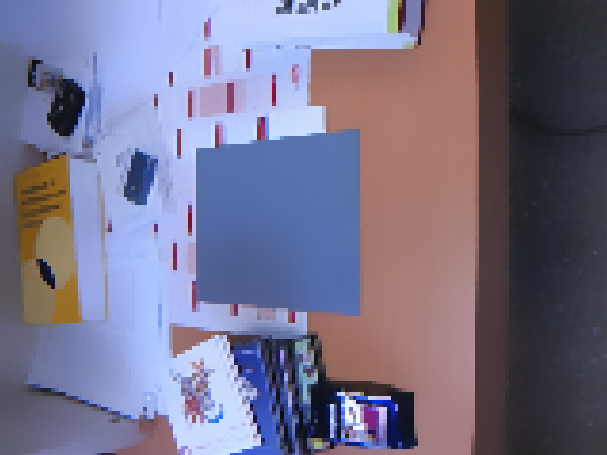
\includegraphics[width = 0.27\textwidth]{Chapters/Images/rs1}&
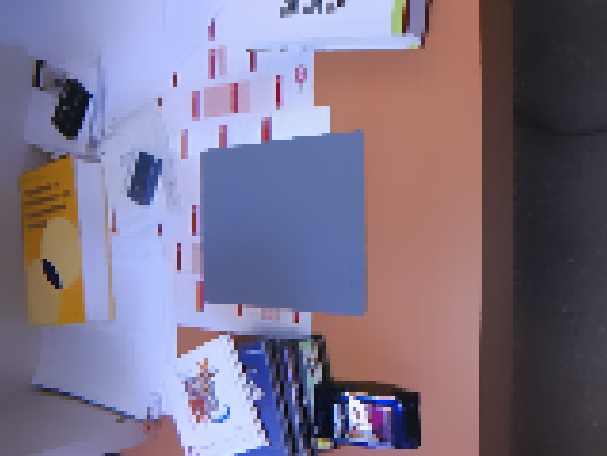
\includegraphics[width = 0.27\textwidth]{Chapters/Images/rs2}&
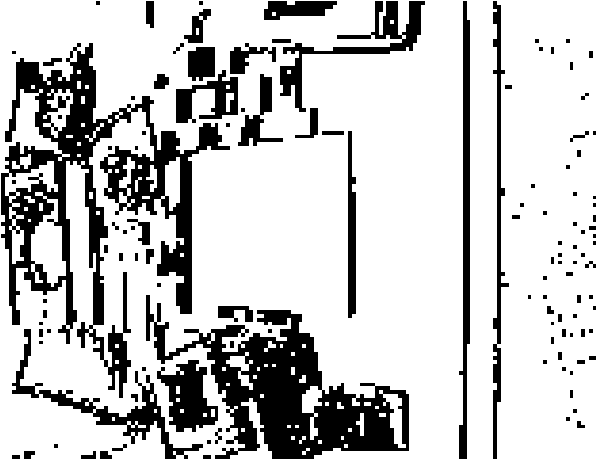
\includegraphics[width = 0.27\textwidth]{Chapters/Images/rs3}
\end{tabular}
\caption{Deux images successives, et le \textit{robust set} qui en découle}
\label{fig_robust}
\end{figure}

\subsection{Carte d'ajustement}
\subsubsection*{Initialisation de la carte}
La carte d'ajustement est initialisée pour tout les pixels appartenant au \textit{robust set} précédemment calculé. Cette initialisation consiste à ajouter à la carte d'ajustement de l'image précédente la différence de couleur entre les deux images. De cette manière, un décalage graduel de la tonalité est compensé.

\begin{equation}
\hat{A}_{i+1}(x) = 
\begin{cases}
A_{i}(x) + (f_{i}(x) - f_{i+1}(x)) & \text{for each} x \in R_{i/i+1}\\
0 & \text{else}
\end{cases}
\end{equation}

\subsubsection*{Complétion de la carte}

Pour les pixels qui ne font pas partie du \textit{robust set}, les auteurs partent du principe que les fluctuations tonales sont globales, c'est à dire que les modifications sont les même pour toute l'image.
Ainsi, les auteurs proposent d'utiliser les ajustements présents dans l'initialisation de la carte pour interpoler les valeurs manquantes. Afin de réaliser cela, les valeurs manquantes sont une moyenne pondérée des ajustements déjà présents.

\begin{equation}
A_{i+1}(x) = \frac{\sum_{r=0}^{N}{w(x,x_{r})\hat{A}_{i+1}(x_{r})}}{\sum_{r=0}^{N}{w(x,x_{r})\chi_{\hat{A}_{i+1}(x_{r})}}}
\label{eqn_aipun}
\end{equation}


$\chi_{A_{i+1}} \equiv R_{i/i+1}$, et $w(a,b) = exp(-\frac{||c(a)-c(b)||^2}{2\sigma_{c}^{2}})$, $c(x)$ étant la couleur du pixel $x$ dans l'espace couleur CIE Lab. Le passage dans l'espace couleur CIE Lab permet de considérer des distance entre couleurs qui ont un sens en regard de la perception des couleurs.\\

On peut réécrire l'équation \ref{eqn_aipun} sous la forme matricielle \ref{eqn_aipun_mat} :

\begin{equation}
A_{i+1}(x) = \frac{W\hat{A}_{i+1}}{W\hat{\chi}_{A_{i+1}}}
\label{eqn_aipun_mat}
\end{equation}

On note que la matrice $W$ est de taille $N\times N$. Elle est donc très coûteuse à calculer. De plus, l'évaluation de \ref{eqn_aipun_mat} est coûteuse. Les auteurs proposent d'utiliser la méthode Nyström \cite{fowlkes2004spectral} afin de calculer une approximation de $W$ : $\tilde{W} = U\tilde{D}U^{T}$ avec $\tilde{D}$ une matrice diagonale contenant les plus grandes valeurs propres de $W$ .

Ainsi on a : 

\begin{equation}
A_{i+1}(x) \approx \frac{U\tilde{D}U^{T}\hat{A}_{i+1}}{U\tilde{D}U^{T}\hat{\chi}_{A_{i+1}}}
\end{equation} 

\subsection{Ré-échantillonnage et alignement tonal}
Enfin, l'alignement tonal consiste à appliquer la carte d'ajustement tonal à la séquence d'image. Dans le cas ou une paire d'images de référence à été choisie, on applique les carte d'ajustements de chaque image de référence sur la séquence d'images, et on fusionne les deux séquences d'image résultantes selon la distance à l'image de référence.


\begin{figure}[h]
\centering
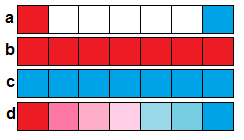
\includegraphics[width=0.5\textwidth]{Chapters/Images/alignement}
\caption{a. Séquence de départ avec ancres, b. Séquence alignée sur l'ancre rouge, c. Séquence alignée sur l'ancre bleue, d. Séquences b et c fusionnées}
\end{figure}